\documentclass[12pt]{ximera}
\title{Practice Exam 1}
\begin{document}
\begin{abstract}
Practice for Exam 1, covering Sections 7.1--7.3: set identities and Venn diagrams,
disjoint sets and complements, inclusion-exclusion, and reading probabilities and
odds off a completed three-set Venn diagram.
\end{abstract}
\maketitle

\section*{Practice Exam 1}

Give your answers as exact fractions, decimals, or percentages; do not round unless
specifically asked to do so.

Formulas that may be useful:
\[
n(A\cup B) = n(A) + n(B) - n(A\cap B), \qquad
P\!\left(\olsi{E}\right)=1-P(E).
\]

\begin{problem}
Assess whether each of the following claims is true or false.

\begin{prompt}
\textbf{(a)} Claim: the union of two sets can be equivalently written as the
complement of their intersection. That is, for sets $A$ and $B$,
\[ A\cup B = \olsi{A\cap B}. \]

\begin{multipleChoice}
\choice{True}
\choice[correct]{False}
\end{multipleChoice}

\begin{hint}
Compare the claim carefully with De Morgan's laws. Is it the sets themselves being
unioned on the left, or their complements?
\end{hint}

\begin{feedback}
False. De Morgan's law says
\[ \olsi{A\cap B} = \olsi{A}\cup\olsi{B}, \]
which is the union of the \emph{complements} --- not $A\cup B$.

For a concrete counterexample, take $\mathcal{U}=\set{1,2}$ and $A=B=\set{1}$. Then
$A\cup B=\set{1}$, while $A\cap B=\set{1}$ and so $\olsi{A\cap B}=\set{2}$. The two
sides differ, so the claim is false.
\end{feedback}
\end{prompt}

\begin{prompt}
\textbf{(b)} Claim: the following Venn diagram shows the set
$\left(\olsi{A}\cap B\right)\cup C$.

\begin{center}
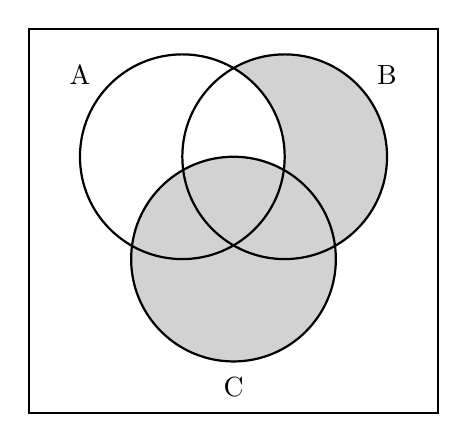
\begin{tikzpicture}[scale=1.3]
  \begin{scope}
    \clip (1,0) circle (1);
    \fill[gray!35,even odd rule] (-1.5,-2.5) rectangle (2.5,1.25) (0,0) circle (1);
  \end{scope}
  \begin{scope}
    \clip (0.5,-1) circle (1);
    \fill[gray!35] (-1.5,-2.5) rectangle (2.5,1.25);
  \end{scope}
  \draw[thick] (0,0) circle (1) node at (-1,0.8) {A};
  \draw[thick] (1,0) circle (1) node at (2,0.8) {B};
  \draw[thick] (0.5,-1) circle (1) node at (0.5,-2.25) {C};
  \draw[thick] (-1.5,-2.5) rectangle (2.5,1.25);
\end{tikzpicture}
\end{center}

\begin{multipleChoice}
\choice[correct]{True}
\choice{False}
\end{multipleChoice}

\begin{feedback}
True. The shading consists of two pieces: the part of $B$ lying outside $A$, and all
of $C$.

The part of $B$ outside $A$ is exactly $\olsi{A}\cap B$, so the whole shaded region
is $\left(\olsi{A}\cap B\right)\cup C$, matching the claim. Note that the union with
$C$ re-shades the portion of $A$ that lies inside $C$, which is why part of $A$ is
shaded even though $A$ is complemented in the first piece.
\end{feedback}
\end{prompt}
\end{problem}

\begin{problem}
Suppose $\mathcal{U}=\set{0,1,2,3,4,5,6,7,8,9,10}$. Consider the sets
\[
A= \set{0,2,4,6,8},\quad B= \set{0,3,6,9},\quad C= \set{1,2,3,4,5},\quad D= \set{7,8,9,10}.
\]

\begin{prompt}
\textbf{(a)} Which of the above sets, if any, are disjoint?

\begin{multipleChoice}
\choice{$A$ and $D$}
\choice{$B$ and $C$}
\choice{$B$ and $D$}
\choice[correct]{$C$ and $D$}
\choice{None of these}
\end{multipleChoice}

\begin{hint}
Two sets are disjoint when they share no elements at all --- their intersection is
empty. Check each pair.
\end{hint}

\begin{feedback}
Check each pair:
\[
A\cap D=\set{8},\quad B\cap C=\set{3},\quad B\cap D=\set{9},\quad C\cap D=\varnothing.
\]
Only $C$ and $D$ have nothing in common, so they are the disjoint pair.
\end{feedback}
\end{prompt}

\begin{prompt}
\textbf{(b)} Which of the following are elements of the set $\olsi{B\cup D}$?

\begin{selectAll}
\choice{$0$}
\choice[correct]{$2$}
\choice[correct]{$4$}
\choice{$6$}
\choice{$8$}
\choice{$10$}
\end{selectAll}

\begin{hint}
Build $B\cup D$ first, then ask which of the listed numbers are \emph{not} in it.
\end{hint}

\begin{feedback}
First, $B\cup D=\set{0,3,6,9}\cup\set{7,8,9,10}=\set{0,3,6,7,8,9,10}$.

Its complement within $\mathcal{U}$ is
\[ \olsi{B\cup D}=\set{1,2,4,5}. \]
Of the listed options, only $2$ and $4$ belong to it. ($0$, $6$, $8$, and $10$ all
appear in $B\cup D$, so they are excluded.)
\end{feedback}
\end{prompt}
\end{problem}

\begin{problem}
Suppose that in a survey of $50$ students, $27$ report they like turtles and $36$
report they like hedgehogs; $19$ of the students report they like both.

\begin{prompt}
\textbf{(a)} Use the Principle of Inclusion-Exclusion to determine how many students
reported liking one or both of these animals.

$\answer{44}$ students.

\begin{feedback}
\[
n(T\cup H)=n(T)+n(H)-n(T\cap H)=27+36-19=44.
\]
\end{feedback}
\end{prompt}

\begin{prompt}
\textbf{(b)} How many students reported liking neither of these animals?

$\answer{6}$ students.

\begin{feedback}
Everyone not counted in part (a) likes neither:
\[ 50-44=6 \text{ students.} \]
\end{feedback}
\end{prompt}
\end{problem}

\begin{problem}
Human blood can contain the A antigen, the B antigen, or the Rh antigen, in any
combination. The following questions involve data about the antigens in patients'
blood as recorded at a particular hospital.

\begin{itemize}
    \item $25$ patients had the A antigen;
    \item $27$ had the B antigen;
    \item $30$ had the Rh antigen;
    \item $17$ had A and B antigens;
    \item $22$ had the B and Rh antigens;
    \item $16$ had Rh and A antigens;
    \item $15$ had all three antigens;
    \item $12$ had none of the antigens.
\end{itemize}

\begin{prompt}
\textbf{(a)} Complete the Venn diagram. Work from the center outward.

\begin{center}
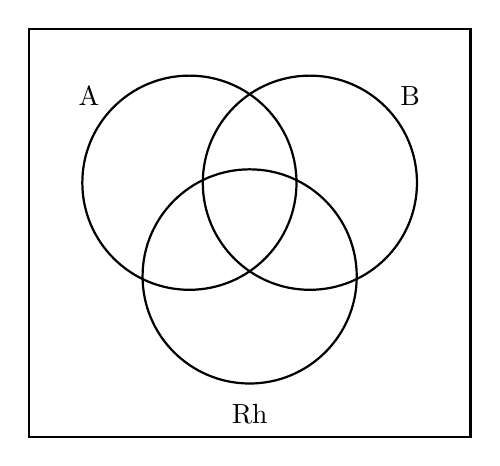
\begin{tikzpicture}[scale=0.85]
  \draw[thick] (-0.9,0.5) circle (1.6) node at (-2.4,1.8) {A};
  \draw[thick] (0.9,0.5) circle (1.6) node at (2.4,1.8) {B};
  \draw[thick] (0,-0.9) circle (1.6) node at (0,-2.95) {Rh};
  \draw[thick] (-3.3,-3.3) rectangle (3.3,2.8);
\end{tikzpicture}
\end{center}

All three: $\answer{15}$

\smallskip
A and B only: $\answer{2}$ \qquad
A and Rh only: $\answer{1}$ \qquad
B and Rh only: $\answer{7}$

\smallskip
A only: $\answer{7}$ \qquad
B only: $\answer{3}$ \qquad
Rh only: $\answer{7}$ \qquad
None: $\answer{12}$

\begin{hint}
The center is given directly. Each two-antigen count includes the people who have all
three, so subtract $15$ from each of them first.
\end{hint}

\begin{feedback}
Working outward from the center:
\begin{itemize}
\item All three: $15$.
\item A and B only: $17-15=2$. \quad A and Rh only: $16-15=1$. \quad
      B and Rh only: $22-15=7$.
\item A only: $25-(2+1+15)=7$. \quad B only: $27-(2+7+15)=3$. \quad
      Rh only: $30-(1+7+15)=7$.
\item None: $12$, given.
\end{itemize}
\end{feedback}
\end{prompt}

\begin{prompt}
\textbf{(b)} How many patients were there total?

$\answer{54}$ patients.

\begin{feedback}
The seven regions inside the circles total
\[ 15+2+1+7+7+3+7=42, \]
and $12$ more patients had no antigens, so there were $42+12=54$ patients.
\end{feedback}
\end{prompt}

\begin{prompt}
\textbf{(c)} Based on this data, what was the probability that a patient would have
all three of the antigens in their blood?

Give your answer as a fraction in lowest terms: $\answer{5/18}$

\begin{feedback}
\[
P(\text{all three})=\frac{15}{54}=\frac{5}{18}\approx 0.278.
\]
\end{feedback}
\end{prompt}

\begin{prompt}
\textbf{(d)} Based on this data, what are the odds that a random person has Rh
antigens? Reduce your answer.

The odds are $\answer{5}$ to $\answer{4}$.

\begin{hint}
Odds compare the number of ways the event happens to the number of ways it does
\emph{not} --- not to the total.
\end{hint}

\begin{feedback}
$30$ patients had the Rh antigen, and $54-30=24$ did not. So the odds are
\[ 30:24 = 5:4. \]
Note the contrast with probability, which would be $\frac{30}{54}=\frac{5}{9}$: odds
put the non-occurrences in the second slot, while probability puts the total there.
\end{feedback}
\end{prompt}
\end{problem}

\end{document}
